%% Copernicus Publications Manuscript Preparation Template for LaTeX Submissions
%% ---------------------------------
%% This template should be used for copernicus.cls
%% The class file and some style files are bundled in the Copernicus Latex Package, which can be downloaded from the different journal webpages.
%% For further assistance please contact Copernicus Publications at: production@copernicus.org
%% https://publications.copernicus.org/for_authors/manuscript_preparation.html


%% Please use the following documentclass and journal abbreviations for discussion papers and final revised papers.

%% 2-column papers and discussion papers
\documentclass[journal abbreviation, manuscript]{copernicus}



%% Journal abbreviations (please use the same for discussion papers and final revised papers)

% The Cryosphere (tc)



% \usepackage commands included in the copernicus.cls:
%\usepackage[german, english]{babel}
%\usepackage{tabularx}
%\usepackage{cancel}
%\usepackage{multirow}
%\usepackage{supertabular}
%\usepackage{algorithmic}
%\usepackage{algorithm}
%\usepackage{amsthm}
\usepackage{float}
\usepackage{subfig}
%\usepackage{rotating}


\begin{document}

\title{Pattern-forming instabilities: feedbacks in the coupling of ice sheets and subglacial drainage systems}


% \Author[affil]{given_name}{surname}

\Author[1]{Arran}{Whiteford}
\Author[2]{Christian}{Schoof}

\affil[1]{Victoria University of Wellington}
\affil[2]{University of British Columbia}


%% The [] brackets identify the author with the corresponding affiliation. 1, 2, 3, etc. should be inserted.



\runningtitle{TEXT}

\runningauthor{TEXT}

\correspondence{Arran Whiteford (arran.whiteford@vuw.ac.nz)}



\received{}
\pubdiscuss{} %% only important for two-stage journals
\revised{}
\accepted{}
\published{}

%% These dates will be inserted by Copernicus Publications during the typesetting process.


\firstpage{1}

\maketitle

\begin{abstract}

 Sharp changes in the basal slipperiness of an ice sheet do not always have a clear source. By modelling instabilities in the coupling of an ice sheet and its subglacial drainage system, we provide a potential mechanism for the formation of such sharp spatial patterns in basal slipperiness and ice flow. These patterns develop to form periodic subglacial lakes and `sticky spots', localised regions of high basal friction.  The instability that forms this structure is driven by a feedback between ice thickness and the subglacial drainage system. Periodic growing humps in ice thickness redirect subglacial water to slippery spots, which in turn increase ice flux into the ice humps. These unstable conditions require a bed permeability weakly dependent on water pressure changes, negligible bed slopes, and a water velocity much greater than ice velocity. 
\end{abstract}


%  Sharp changes in the basal slipperiness of an ice sheet do always have an clear source. By modelling instabilities in the coupling of an ice sheet and subglacial drainage system, we describe physical feedback mechanisms that force the formation of sharp spatial patterns in basal conditions and ice flow. This model predicts the spontaneous formation of  periodic subglacial lakes and `sticky spots', localized regions of high basal friction.  While previous research depicts similar structures through empirical and modelled descriptions, we describe the spontaneous formation of such spatial structure. The instability that forms this structure is driven by a feedback between variations in ice thickness, and basal slipperiness.  Periodic growing humps in ice thickness redirect subglacial water to slippery spots, which in turn increase ice flux into the ice humps, so they continue to grow.
% Scaling a one--dimensional model ice sheet coupled to a basal drainage system, we find conditions for the instability with linear stability analysis. Solutions in the full nonlinear model are simulated  numerically,  using operator splitting and finite difference methods. The instability requires a bed permeability weakly dependent on water pressure changes, negligible bed slopes, and a water velocity much greater than ice velocity. The `sticky spot'--lake pairs are predicted to form with periodic spacing and migrate upstream. 


\copyrightstatement{Copyright Authors 2019 This work is distributed under
the Creative Commons Attribution 4.0 License.}


\introduction  %% \introduction[modified heading if necessary]
 Faster flowing ice discharges more ice from the centre of an ice sheet to the sea, affecting ice mass budget and global sea level. The speed of ice flow depends strongly on its coupling with the underlying bedrock \citep[e.g.][]{rose1979characteristics,engelhardt1990physical}. Changes in friction at this interface can drastically affect ice flux rates by allowing ice to stick or slide on the bed \citep{budd1979empirical}. Subglacial water is thought to be fundamental to this process:
 pressurised water underneath an ice sheet decouples ice from the bed, reducing friction and allowing ice to slide \citep{weertman1957sliding,iken1986combined, alley1989water}. This can be seen in the fast flowing ice streams of Antarctica, which overlie pressurised, saturated sediment slurries \citep{blankenship1986seismic, alley1986deformation, alley1987till,  robin1970radio, engelhardt1997basal,kamb2001basal, hodson2016physical}. While ice streams are relatively small in area, they contribute 90 \% of the total dynamical ice loss from  Antarctica \citep{bamber2000widespread, rignot2011ice}, and so are a key determinant of the continent's ice budget. 

% Antarctic basal conditions are completely disconnected from seasonal surface changes \citep{ashmore2014antarctic}, but can vary dramatically in space and time,. Some observed temporal and spatial changes in basal friction or subglacial drainage are thought to be caused by varying basal conditions or by feedbacks within the ice sheet: for instance, the feedback driving fast flowing ice streams \citep{bennett2003ice,kyrke2014subglacial}, the spatial patterning of ice stream formation \citep{fowler1996ice}, ice stream stagnation \citep{alley1994water},  or reoccurring subglacial floods \citep{wingham2006rapid}. In this paper we examine pattern forming feedbacks between ice sheets and subglacial drainage systems

There is indirect evidence that changes in basal conditions in regions of the Antarctic 
ice sheet have a striped pattern, with stripes being oriented at 
right angles to ice flow.  \citet{sergienko2013regular}, and \citet{sergienko2014similarity} discovered distinctive laterally symmetric patterning in the driving and basal stresses in regions of Antarctica and Greenland. 
In an empirical study based on multiple remote--sensing techniques, \citet{fricker2010synthesizing} found repeating subglacial lakes coinciding with sticky spots, and hypothesise that the lakes are formed as the result of feedbacks with basal shear stress, hydraulic gradients and ice flux, as described by \cite{sergienko2007causes}. In theory, a sticky spot slows down ice, forming an ice hump. Ice then accelerates and thins on the downstream side of the hump, creating a low in hydraulic gradient, causing water ponding and subglacial lake formation. This feedback is modelled by \cite{sergienko2011sticky} who  prescribe a sticky spot and predict subsequent lake formation. Correspondingly, \citet{pattyn2003new} model the thinning of ice as it flows over an existing lake. Both `sticky spots' and subglacial lakes are thought to play important roles in ice stream dynamics: `sticky spots' have been found to modulate ice stream flow \citep{winberry2011dynamics}, providing basal shear stress, while it has been hypothesised that subglacial lakes could catalyse ice stream inception \citep{livingstone2013potential}. 

To date, there is no evidence of water storage structures forming quasi--periodic patterns. The only confirmed examples of spatial patterning in ice sheets are found in the bed of paleo--ice sheets, which present a variety of well documented sediment patterns, for instance, drumlins or bed ribs  \citep[e.g.][]{ kinahan1872general, hattestrand1997ribbed}, modelled by \citet{hindmarsh1998stability,hindmarsh1998ice, fowler2000instability, schoof2007pressure, dunlop2008bed,fowler2014instability}.
In order for bed topography to be transmitted to the surface it must have a wavelength greater than ice thickness  \citep{gudmundsson2003transmission}. It is therefore plausible that these sediment patterns could give rise to significant surface expressions on the ice sheet such as those on observed by \citet{sergienko2014similarity}.

Most empirical observations of subglacial water in Antarctica are related to documenting subglacial lakes \citep[e.g.][]{carter2007radar,wright2012fourth,siegfried2018thirteen}. The vast majority of documented lakes are large permanent features formed by topographical basins \citep{wright2012fourth}. However, flat--bedded water storage features continue to be found in more detailed surveys: \citet{carter2007radar} and \citet{young2016distribution} describe numerous features they suspect may indicate saturated sediments or ``swamps''. Similarly, Lake Whillans is thought to be a poorly defined swamp--like lake that fills and drains dynamically, and is formed in a very shallow basin about $6 \mathrm{ m}$ deep \citep{horgan2012subglacial}. 

This research expands on the work of \citet{sergienko2011sticky} and \citet{sergienko2014similarity}. While we do not attempt to describe the specific patterned structures found by \citet{sergienko2014similarity}, we attempt to show that feedbacks between ice flow and subglacial drainage can cause the spontaneous formation of patterned spatial structure and even lake formation. By using a model with a coupled ice sheet and subglacial drainage system, we find conditions for which a pattern--forming instability could exist, show that localised water ponding increases without bound until ice starts to float, and  deduce a mechanism for the positive feedback. 
%This corresponds to the instability described by \citet{sergienko2011sticky}, but with a key improvement: our model shows the spontaneous growth of the structure described. 

The mechanism that forces the growth of spatial structure is driven by feedbacks in the coupling of ice sheet and subglacial drainage.
While the weight of a changing ice sheet affects the distribution and routing of subglacial water, the subglacial water in turn changes the flow of ice due the effect of water pressure on sliding friction. Lastly, the speed of the ice and ice thickness  are linked through continuity. The instability relies on a slight phase shift between striped basal conditions and oscillating ice thickness: regions of faster flowing ice must extend into ice humps to make them grow. 

Few previous studies have looked at feedbacks in this coupling in detail. This may be an issue of scales:
It is common to assume that drainage is much faster than ice flow, and
so while velocity and drainage are tightly coupled, it is easy to ignore the effect of an evolving surface topography on drainage in detail, assuming instead that ice geometry can be treated as fixed at 
the time scale on which the drainage system evolves \citep[e.g.][]{hindmarsh1998stability,fowler2000instability,schoof2014oscillatory}.

\section{1D coupled ice sheet--drainage model}

%\subsection{Introducing the model} \label{sec:model}

We model a simple one--dimensional ice sheet coupled to a basal drainage system using three equations. $x$ is the  position along the flowline in the downstream direction, oriented parallel to the bed, while $t$ is time (Fig. \ref{fig:domain}). The model's three dependent variables are ice velocity $u(x,t)$, ice thickness $h(x,t)$ and 
effective pressure $N(x,t)$ defined as the difference between the pressures of overburden ice and subglacial water.    
The model's spatial domain covers a section of the flowline, and is small relative to the size of an ice sheet but large relative to ice thickness. This scale allows us to make certain simplifying assumptions:
by modelling a relatively short subsection of the ice sheet, we can apply periodic 
boundary conditions, assuming that the next similarly--sized subsection of 
the ice sheet effectively behaves the same as the subsection under
consideration.
The large length--to--depth ratio allows us to assume vertical velocities are negligible compared to the horizontal. Negligible vertical velocities allow us to use a depth--integrated ice flux divergence.


\begin{figure}[hbt!]
\centering
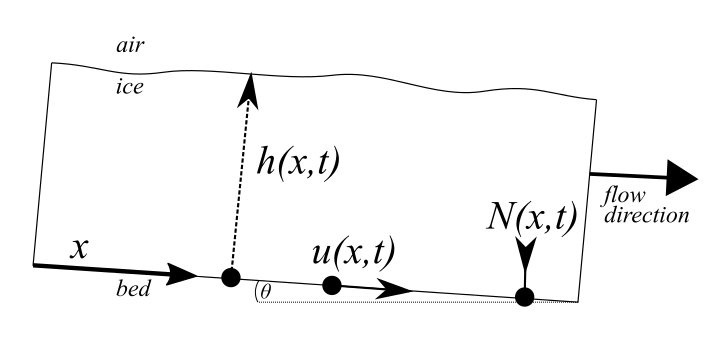
\includegraphics[width=0.7\textwidth]{pictures/domain.png}
\caption[Schematic of the model domain]{The domain is a one dimensional section of ice along the flowline, where $x$ is distance along the bed in the downstream direction. Three variables ice thickness $h$, ice velocity $u$ and effective pressure $N$ are modelled along the domain. $\theta$ is the angle of the bed from the horizontal.}
\label{fig:domain}
\end{figure}

We also assume that sliding dominates internal deformation as a mechanism for ice transport. This justifies our assumption that the velocity $u$  
depends only on horizontal position $x$ and time $t$, but not on distance 
above the bed.
The appropriate depth--integrated 
form of the Stokes equations in this case is \citep{macayeal1989large, schoof2010thin}

\begin{equation} \label{eq_1}
4 (\eta h u_x)_x - \tau_b (u,N) - \rho g h ( h_x - \sin \theta ) = 0.
\end{equation}
$4(\eta h u_x)_x$ is the gradient 
of depth--integrated extensional stress in the ice, where $\eta$ is 
viscosity and subscripts $_x$ and $_t$ denote partial derivatives. 
$\tau_b(u,N)$ is friction at the base of the 
ice sheet, which we assume depends on sliding velocity $u$ and  
effective pressure $N$. The justification for such a friction law can be 
found either in the classical theory of sliding over hard beds \citep{lliboutry1968general, budd1979empirical, bindschadler1983importance, fowler1986sliding, fowler1987sliding}
or 
in models of basal motion facilitated by a layer of water--saturated, 
deforming till \citep{blankenship1987till, boulton1987sediment, kamb1991rheological, iverson1998ring}.
Common to specific friction laws describing these two modes of
sliding is that friction is a non-decreasing function of sliding 
velocity ($\partial \tau_b/\partial u \geq 0$), and that friction 
increases with effective pressure ($\partial \tau_b/\partial N > 0$). A 
commonly used (though by no means unique) model that satisfies these 
constraints is the friction law sometimes referred to as a `Generalised Weertman Sliding Law'
$$ \tau_b = C u^a N^b, $$
with $b$ and $C$ positive and $a$ non--negative.  The dependence on 
effective pressure is key to our model as it couples ice flow to the subglacial drainage system. For hard beds, a lower effective 
pressure implies water can more easily force its way between ice 
and bed, causing larger water--filled cavities to form. These reduce 
ice--bed contact and therefore reduce the amount of friction at the bed. For
deformable beds, a lower effective pressure reduces contact forces 
between sediment grains and allows them to move past each other more 
easily.
The last term in equation \eqref{eq_1} is the `driving 
stress', equal to the depth--integrated sum of the downslope component of 
gravity and bed--parallel
cryostatic pressure gradient. These describe the pull of gravity on ice both down the bed slope and in flattening the ice sheet surface. Here $\theta$ is the bed slope, $\rho$ is 
the density of ice and $g$ is acceleration due to gravity.

We assume that accumulation and melting of 
ice are negligible at the length scales of interest, so that 
depth--integrated mass conservation can be written as
\begin{align} \label{eq_2}
h_t + (hu)_x = 0.
\end{align}

Lastly, we couple the ice sheet model with a subglacial drainage system by describing the conservation of water as it is flows under the ice:
\begin{align} \label{eq_3}
 {h_w}_t (N) +  {q_w}_x = 0, \\
   q_w = \kappa (N) \psi , \qquad \psi = \rho_w g \sin\theta + N_x - \rho g h_x,
\end{align}

where $q_w$ and $\rho_w$ are the flux and density of water respectively, and $\psi$ is hydraulic gradient.

Equation \eqref{eq_3} assumes there is no water supply within the domain from the melting of ice or surface runoff reaching the bed.
Water flux is given by a form of Darcy's law $ q_w = \kappa (N) \psi $, which is  used to describe fluid flow through a porous medium: flux is forced by hydraulic gradient $\left( \rho_w g \sin\theta + N_x - \rho g h_x  \right)$ and restricted by the depth--integrated permeability $\kappa(N)$ of the water--filled till column   \citep[e.g.][]{bear2013dynamics, hillel2013fundamentals}. 
Permeability of a sublacial till layer depends on porosity, which decreases with compression. It follows that we expect $\kappa$ to be a decreasing 
function of $N$ ($\partial \kappa / \partial N \leq 0$), for instance $\kappa(N) = \kappa_0 e^{-mN}$.
Changes in porosity are similarly related to $h_w$, water storage per unit area of the bed: larger pores relate to more water storage. $h_w$ is assumed to be a function of effective pressure $h_w=h_w(N)$ which has a negative derivative $\partial h_w(N) / \partial N < 0$, for example $h_w(N) = {h_w}_0 e^{-dN}$. 

While the drainage model \eqref{eq_3} can describe flow through subglacial till, it can also serve as a model 
for flow along the ice--till interface through a `sheet' as proposed by \citet{schoof2012flotation} and \citet{hewitt2012flotation}. This is approximately true if the sheet thickness evolves much faster than the water storage, where the 
sheet thickness ($h$ in the notation of these papers) is a function of 
effective pressure $N$ and sliding velocity $u$. If we use a simplified 
model in which sliding velocity is a function of effective pressure, then
sheet thickness and the resulting permeability are also decreasing 
functions of effective pressure. In any case, the minimal 
assumptions that our model rests on are that water storage at the bed or 
in basal ice just above the bed \citep{werder2013modeling, schoof2014oscillatory}
decreases with effective pressure (or equivalently, increases with basal 
water pressure), and that water flow is driven by the hydraulic gradient 
$\psi$, modulated by a permeability that can be either constant or 
decrease with effective pressure.
\citet{alley1996towards} makes equivalent assumptions about the prescribed relationships between flux, water storage, and the ability of the system to transmit water in a `sheet flow' distributed drainage model that is commonly used in large scale ice sheet models \citep{flowers2015modelling}. 

The model described above couples the flow of ice, changes in ice thickness and 
the flow of water at the bed. The feedbacks in this coupling drive an instability in the model and the spontaneous 
formation of spatial structure. This process can be visualised as follows: Take a spatial perturbation to an 
initially uniform effective pressure distribution. Consider a location where $N$ is reduced. On its own, this would lead to reduced basal 
friction $\tau_b(u,N)$, but in practice, we expect that $u$ will 
increase in the same locations, either to counterbalance the effect of 
$N$ on $\tau_b$, or to provide sufficiently large extensional stress gradients. A localised increase in $u$ will lead to mass transport away 
from the same location, presumably leading to a positive perturbation in 
ice thickness downstream of the location of reduced effective pressure.  
This surface perturbation in turn affects the hydraulic gradient 
that drives water flow. In fact, from this sketch, it is conceivable 
that a local depression in $N$ leads to a positive ice thickness 
gradient downstream, which corresponds to a reduction in hydraulic 
gradient $\psi$ and therefore to a reduction in water flow out of the 
depression in $N$. This should then cause water to accumulate in that 
depression, further lowering $N$. Our primary aim in what follows is to 
investigate mathematically whether there are conditions under which a 
positive feedback of this type can indeed operate and lead to the emergence of 
spatial structure in basal water pressure, ice velocity, and surface 
elevation. We do so by investigating the stability of the trivial, 
spatially uniform solution to equations \eqref{eq_1}--\eqref{eq_3} with respect to 
small perturbations by means of a linear stability analysis. 
Subsequently, we address whether finite perturbations can grow 
sufficiently for ice to begin to float, and separate from the bed.

The remainder of this paper is organised as follows:
Firstly, we scale the model to a dimensionless form. Secondly, we analyse the stability of a steady state solution and find parameter 
regimes and wavelengths that support instability by performing a linear stability analysis. Thirdly, we examine features of a unstable linear solution and deduce the mechanism driving the instability. Lastly, we introduce a numerical solver and show the longer term evolution of a nonlinear solution in a regime that forces instability.

\subsection{Non--dimensionalisation of the model} \label{sec:scaling_the_model}
For each variable in our model, we define a scale (or natural 
unit), denoted by the symbol for the variable in square brackets (e.g. $[x]$). 
We then define 
a dimensionless version of each variable by scaling as

\begin{align}
x^*=\frac{x}{[x]},\quad t^*=\frac{t}{[t]},\quad
u^*=\frac{u}{[u]}, \quad h^*=\frac{h}{[h]},\quad
N^*=\frac{N}{[N]}  \label{scales}
\end{align}

\begin{align}
\tau_b^*(u^*,N^*)=\frac{\tau_b(u,N)}{\tau_b([u],[N])} , \quad 
\kappa^*(N^*)=\frac{\kappa(N)}{\kappa([N])}, \quad 
h_w^*(N^*)=\frac{h_w(N)}{h_w([N])}. \quad 
\end{align}

$[h]$ is prescribed from initial conditions
as the mean ice thickness.
Assume that the mean flux  of  water $\bar{Q}$ through  the  domain  is  given,  at  least  initially.   This  allows  us  to  define  the remaining scales  $[N]$, $[u]$, $[x]$ and 
$[t]$ through the scale relations
\begin{subequations}
\begin{align} 
%\kappa([N])\rho_w g \sin \theta & = \bar{Q},\\
\frac{[N]}{[x]^2} &= \rho_w g \frac{[h]}{[x]^2}, \label{scale_2}\\
{\tau_b([u],[N])}&=\rho g [h] \sin (\theta), \label{scale_3}\\
\frac{[h]}{[t]}&=\frac{[h][u]}{[x]}, \label{scale_4}\\ 
\frac{h_w([N])}{[t]}&=\frac{\kappa([N])[N]}{[x]^2} \label{scale_5}.
\end{align}
\end{subequations}

To compute the remaining scales we do the following: Given a mean 
ice thickness $[h]$, $[N]$ can then be computed if we require that the contribution of 
effective pressure gradients $[N]/[x]^2$ to hydraulic gradient be 
comparable to the direct effect of changing ice thickness $\rho_w g[h]/[x]^2$ (Equation \ref{scale_2}).
With $[N]$ and $[h]$, a velocity scale $[u]$ can be computed by balancing basal friction with the average
driving stress (Equation \ref{scale_3}).   Lastly, by solving \eqref{scale_4} and \eqref{scale_5} simultaneously we can solve for a length  and advective time scales $[x]$ and $[t]$ respectively. Note that to compute scales explicitly, the functional forms of $\kappa$ and $\tau_b$ need to be prescribed.

We obtain the four dimensionless 
parameters
\begin{align}
\epsilon = \frac{ \eta [u]}{[x]^2  \rho g \sin(\theta) }, \qquad
\delta =  \frac{[x]}{[u][t]}, \qquad 
\gamma = \frac{\rho_w g \sin(\theta) [x] }{[N]}, \qquad  r = \frac{\rho_w}{\rho}, \label{edg}
\end{align}

which we interpret in the 
following way: $\epsilon$ is a dimensionless extensional viscosity, 
$\delta$ is the fraction of the domain ice passes over with the length and timescales $[x]$ and $[t]$, and $\gamma$ is the ratio of the hydraulic gradient driven by bed slope to that driven by diffusion.
 $r$ is a material 
constant, with a fixed value close to unity. 

In 
dimensionless form, omitting the asterisks on the 
dimensionless variables, the model takes the form:

\begin{subequations}
\begin{align}
 4  \epsilon\left( h u_x \right)_x -  \tau_b(u ,N) + h \left(1 - \frac{ \delta}{\gamma} h_x \right)=0, \label{scaled_eq_1}\\
\delta h_t +  (h u )_x = 0, \label{scaled_eq_2}\\
  {h_w}_t(N) + \left( \kappa \left( N \right) \left( \gamma
   + N_x - r \delta h_x \right) \right)_x= 0. \label{scaled_eq_3}
\end{align}
\end{subequations}


%\subsection{Steady State}

We denote the spatially 
uniform steady state solution to equations \eqref{scaled_eq_1}--\eqref{scaled_eq_3} by $u(x,t) 
\equiv \bar{u}$, $h(x,t) \equiv \bar{h}$, $N(x,t) \equiv \bar{N}$, where 
the only non-trivial equation in \eqref{scaled_eq_1} -- \eqref{scaled_eq_3} that must be satisfied 
by the constants $\bar{u}$, $\bar{h}$ and $\bar{N}$ is
$$ \tau_b(\bar{u},\bar{N}) = \bar{h}. $$
Through our choice of scales, we have made sure that 
$\bar{h} = 1$, the mean ice thickness is scaled to unity. 
Additionally, we have set $\bar{N} = 1$ by choosing scales such that dimensionless $N = 1$ corresponds to 
dimensionless $\kappa(N) = 1$, and by requiring a dimensionless mean water flux of unity, where water flux is simply $\kappa(N)$ in the absence of 
gradients in $h$ or $N$. Lastly, we have also ensured through our 
definition of the dimensionless friction law $\tau_b$ that 
$\tau_b(\bar{u},1) = 1$ is solved by $\bar{u} = 1$, so the steady state 
is $(u,h,N) \equiv (1,1,1)$, and in the steady state, $\kappa = \tau_b = 
1$. 

In the next 
sections, we analyse the stability of this trivial steady 
state: if a small perturbation is added to ($\bar{u},\bar{h},\bar{N}$), 
under what circumstances will that perturbation grow? What parameter 
regimes and wavelengths give rise to such growth, or instability? To 
answer this question, we perform a linear stability analysis.

\section{Linear Stability Analysis} \label{sec: lin_stab_ana}
%\subsection{Justify Scale Size  }

 We  focus on the specific parameter regime:
$$ \delta \gg \gamma \gg  1 $$  
which is equivalent to
$$ \rho_w g \sin(\theta) [x]  \gg [N] \gg  \rho_w g \sin(\theta) [u][t].   $$ Physically, this describes a subglacial drainage scheme where the pressure gradient caused by bed slope (hydraulic head) is much greater than effective pressure, in spite of a small bed slope. Additionally, changes in the hydraulic head in the timescale of a model run are relatively small, as ice only travels a small distance in the domain. The choice of this parameter regime is not accidental:  it leads to identification of an instability. In numerical solvers, we use the specific parameters and functions listed in Table \ref{tab:params_dimentionless}.
% $$ \delta/ \gamma \gg 1 \qquad \mathrm{and} \qquad \delta \gg 1 $$.

\begin{table}[hb!]
\centering
\begin{tabular}{||c||} 
 \hline
$\epsilon= 1$  \\ 
 \hline
 $\gamma = 10^{2}$ \\
 \hline
$\delta = 10^{3}$ \\
 \hline
 $\tau_b(u,N)= u^{3/4}N^{3/4}$  \\
 \hline
 $\quad h_w(N)= e^{-N}$ \\ 
 \hline
 $\kappa(N)=e^{-0.0001 N}$\\[1ex] 
 \hline
\end{tabular}
\vspace{10pt}
\caption{Dimensionless parameters and functions used in numerical solutions. This regime is not unique.}
\label{tab:params_dimentionless}
\end{table}
\begin{center}
\end{center}
%\subsection{Scale $h$ and $\kappa$}

Our original model is based on the horizontal length scale of 
interest ($[x]$) being short compared 
with the length $L$ of the ice sheet, so that the tendency of the ice 
sheet to thin at the margins does not appear at 
the scale under consideration, and we can treat the domain as being 
approximately periodic. We have allowed for a finite bed slope $\theta$ 
in order to drive the flow at this scale. In the unperturbed steady 
state, $\theta$ is then also the surface slope, and for a realistic ice 
sheet, the surface slope is comparable with $[h]/L$. One of our scale 
relations, equation \eqref{scale_3}, requires ${[N]}/{[x]^2} = \rho_w g {[h]}/{[x]^2}$. 
Setting $\theta = [h]/L$, we have, with small $\theta$, $[N] \approx 
\rho_w g [h] [x]/[L]$, and the requirement that $[x]$ be much less than 
$L$ translates, roughly, into $[N]$ being much less than the ice 
overburden $\rho_i g[h]$, which is typically required for any kind of 
appreciable sliding \citep{schoof2006variational}.

Given $[x] \ll L$ is then equivalent to $[x]\sin(\theta) \ll [h]$, and 
consequently $\delta \gg 1$ and $\delta/\gamma \gg 1$, all things being equal, an $O(1)$ variation in $h^*$ over an $O(1)$ displacement $x^*$ would lead to a thickness 
gradient that overwhelms all other terms in the force balance \eqref{scaled_eq_3}, and so $h(x, t)$ is constant to leading order.
As a result, we expand $h(x, t)$ as $h(x, t) = h_0 + \delta^{-1} h_1(x, 
t)$, where $h_0$ is then a constant. It is then clear that 
$h_0$ is also the steady state ice thickness, and by our choice of
original scales, we can set $h_0 = \bar{h} = 1$.


Applying the same approach to equation \eqref{scaled_eq_3}, we obtain at leading 
order that
$$ \frac{\partial \kappa}{\partial N} \frac{\partial N}{\partial x} = 0.$$
This allows for two conclusions: either $N$ is spatially uniform, or 
$\partial \kappa / \partial N$ vanishes \emph{at leading order}. The 
former is clearly not interesting, as a uniform $N$ would prevent a 
positive feedback between flow, thickness evolution and drainage to 
arise, in the sense that there cannot be any drainage--driven spatial 
variation in friction $\tau_b(u,N)$ in that case. Consequently, we 
assume instead that permeability $\kappa$ is only weakly dependent on
effective pressure, and specifically, that we can put $\kappa = \kappa_0 
+ \gamma^{-1}  \kappa_1(N)$ with $\kappa_0$ constant. By our choice of 
scales, it then follows that $\kappa_0 = 1$.

At leading 
order in $u$ and $N$ and first order in $h$, the model then reduces to

\begin{subequations}
\begin{align}
4 \epsilon  u_{xx}-\tau_b(u,N) + 1= 0, \label{red_mod_1}\\
 {h_1}_t+ u_x=0 ,\label{red_mod_2} \\
{h_w}_t(N) + \kappa_1(N)_x+  N_{xx} -  r {h_1}_{xx} = 0  .  \label{red_mod_3}
\end{align}
\end{subequations}

Note that the only 
nonlinear part of these equations are the constitutive laws that we 
prescribe: $\tau_b(u,N)$, $ {h_w}(N)$, and $\kappa_1(N)$.
If we were to choose, somewhat unrealistically, linear functions, the
resulting model would be directly solvable by Fourier series without 
further simplification.

%\subsection{Linear stability analysis} \label{sec:Linear stability analysis}

We next analyse the 
stability of the steady state solution $(u,h_1,N) \equiv 
(\bar{u},\bar{h_1},\bar{N}) = (1,0,1)$ of the dimensionless coupled 
ice--flow--drainage model \eqref{red_mod_1}--\eqref{red_mod_3}. The first order (linear) approximation of our model is:

\begin{subequations}
\begin{align}
    0 &= 4\epsilon  u_{xx} - \bar{\tau_b} - {\tau_b}_u u - {\tau_b}_N N+ 1,   \label{lin_eq_1}\\
 {h_1}_t &= -  u_{x}, \label{lin_eq_2}\\
  h_{w N} N_t &= - \kappa_N N_x  - N_{xx} + r  {h_1}_{xx} , \label{lin_eq_3}
 \end{align}
\end{subequations}

where
$$ {\kappa_1}_N = \left.\frac{\partial \kappa_1}{\partial N}\right|_{N = 
\bar{N}}, \qquad {\tau_b}_u = \left.\frac{\partial \tau_b}{\partial 
u}\right|_{u = \bar{u}, N = \bar{N}},  \qquad {\tau_b}_N = 
\left.\frac{\partial \tau_b}{\partial N}\right|_{u = \bar{u}, N = 
\bar{N}}. $$
Note that by construction of the model, we assume that $\kappa_N \leq 
0$, $\tau_u \geq 0$, and $\tau_N > 0$.
Equations \eqref{lin_eq_1}--\eqref{lin_eq_3}
are a set of linear partial differential equations with constant 
coefficients posed on a periodic domain, and can be solved by means of a Fourier series to obtain a generalised eigenvalue problem from which we obtain a dispersion relation  
\begin{align}
\sigma(k)_{1,2}&=\frac{k^2-  i {\kappa_1}_N k  \pm \sqrt{( i {\kappa_1}_N k - k^2)^2-(4 {h_w}_N \frac{i r  \tau_N k^3}{ 4\epsilon  k^2 +\tau_u})}}{2{h_w}_N} \label{dispersion_relation}  
 \end{align}  
which has two roots, $\sigma_1(k)$ and $\sigma_2(k)$.

A single unstable mode $k$ (i.e. a single wavenumber $k$ for 
which it is possible to find a positive growth rate 
$\mathrm{Re}(\sigma)$ for a given set of model parameters) signals 
instability, whereas all wavenumbers must correspond to at least 
non--positive growth rates to assure stability of a steady state solution.
We determine 
numerically the behaviour of $\Re(\sigma)$ over a range of wavenumbers $k$, shown in Figure \ref{fig:sigma_instability}.  
For the parameter regimes described, we can see instability ($\sigma > 0$) for small $k$.  As $k$ grows, the positive growth rate approaches zero. 



\begin{figure}[htb!]
\centering
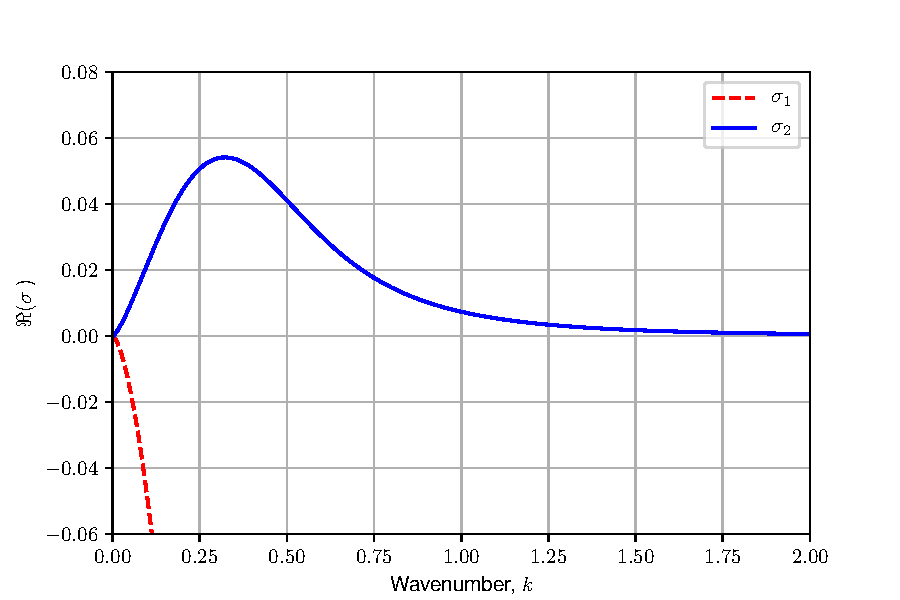
\includegraphics[width=0.7\textwidth]{pictures/dispersion_relation.pdf}
\caption[Growth rates from dispersion relation]{Growth rates $\Re (\sigma_1)$ and $\Re( \sigma_2)$ for a range of wave numbers calculated with the dispersion relation (Equation \eqref{dispersion_relation}). For this parameter regime, the constant steady state is unstable for large wavelengths. Parameters and functions from Table \ref{tab:params_dimentionless}.}
\label{fig:sigma_instability}
\end{figure}


\section{Numerical analysis} \label{sec:numerics}

The linear stability analysis we have just performed confirms that a 
trivial steady state solution can be unstable, in which case we expect 
spatial structure to evolve. We are not able to determine the final 
result of that instability from a linearised theory alone. In 
particular, we want to determine whether the instability could lead to 
the spontaneous formation of larger subglacial water bodies: will the 
instability simply lead to more water being stored in till in some 
locations than in others, or will it actually cause water to accumulate until ice is floating? In order to answer that 
question, the full model must be solved 
numerically. 

The numerical scheme uses operator splitting to solve for each variable at each step separately and sequentially. The parameters and functions used are listed in Table \ref{tab:params_dimentionless}, and initial conditions represent random noise. The scheme is described in detail in the appendix.
The evolution of the solution, shown in Figure \ref{fig:instability_float_1}, sees the development of a  dominant wavelength that continues to grow in amplitude reaching an effective pressure of zero. Most importantly, we see that the instability is not bounded, and a pattern with a characteristic wavelength emerges
early in simulation.
As the perturbations in $N$ and $u$ reach finite amplitude, there is some evidence of nonlinear effects. Rather than evolving as smooth sinusoids, the solution evolves slight asymmetric spatial structure. 

At the time where $N=0$, the developed spatial structure displays localised `sticky spot' regions with high $N$, slow $u$ and thick $h$, followed immediately downstream by `lake' regions with low $N$, large $u$ and thin $h$, followed downstream by more slow flowing ice.

\begin{figure}[htb!]
\centering
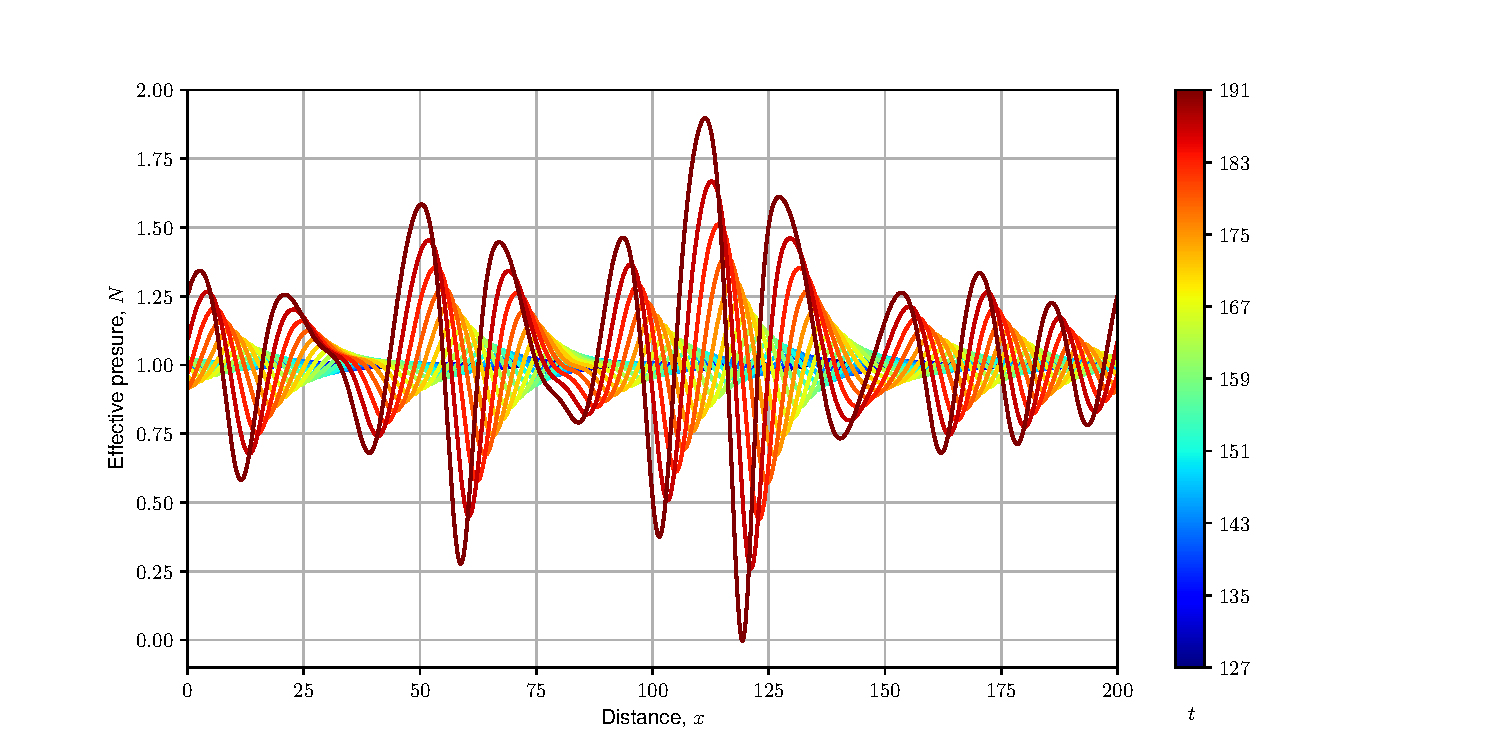
\includegraphics[width=1\textwidth]{pictures/growtofloat.pdf}
\caption[Nonlinear evolution of an unstable solution]{Nonlinear evolution of an unstable solution for effective pressure shows the development of spatial structure: Each line is the solution at a point in time depicted by its colour.  The solution grows until ice reaches the point of flotation $N=0$ where the model breaks down. Lows in effective pressure at $x=15$, $38$, and $77$ would continue to grow in amplitude until they also reach $N=0$.}
\label{fig:instability_float_1}
\end{figure}

The simulation is continued until $N = 0$ is reached, at which point the model breaks down. Mathematically, we cannot continue the computation because the friction law does not in general compute a 
real--valued $\tau_b$. Physically, the model breaks down because $N = 0$ not 
only corresponds to bed friction vanishing, but also to ice separating 
from the bed, and a cavity 
between ice and bed can form, which is not supported by equation \eqref{eq_3}, the subglacial drainage model.

\begin{figure}[htb!]
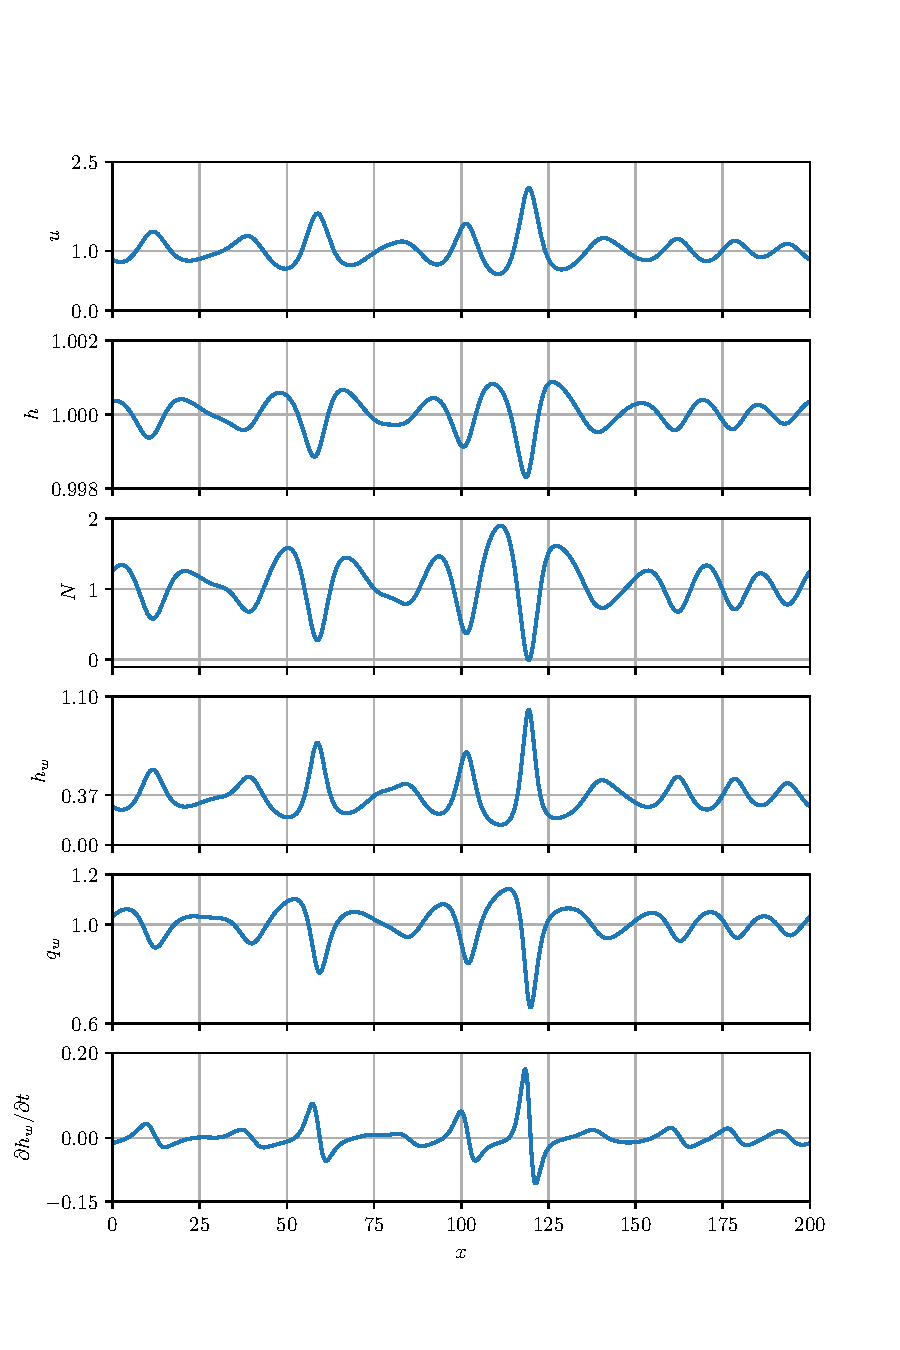
\includegraphics[width=0.65\textwidth]{pictures/solnatfloat.pdf}
   \caption{From top to bottom: velocity $u$, ice thickness $h$, effective pressure $N$, changing water storage $h_{w_t}$, water flux $q_w$ and water storage $h_w$ at distance $x$ accross the domain, corresponding to Figure \ref{fig:instability_float_1} at the point in time where $N$ reaches $0$.}
   \label{fig:solnbreakdown}
\end{figure}


% \subsection{Physical mechanism}
A close look at the unstable model solution reveals why we see growth in the solution's amplitude: 
a phase shift between solution variables drives a positive feedback between ice thickness, velocity and effective pressure. A velocity maximum is shifted slightly downstream of a low in ice thickness, while velocity and effective pressure are roughly antiphase (Figure \ref{fig:schematic_unstable}).  From this we can describe the positive feedback loop:
 A hump of ice slows water flow in the positive 
$x$--direction, with that slowing being most pronounced where the slope perturbation $h_x$ is large and negative. This causes water to accumulate 
upstream of locations of negative slope perturbations, that is, near 
minima of $h$. Because these correspond to minima in $N$, water accumulation 
causes a further drop in $N$, causing the perturbation in $N$ to grow.
The low effective pressure reduces ice--bed friction increasing sliding and creating a high in velocities in this area.
Note that although $N$ and $h$ are approximately in phase, $N$ lags $h$ somewhat. This then causes $u$ to lead $h$ in phase: velocity maxima occur upstream of maxima in $h$, 
causing more ice to flow into the hump of ice than out and so the hump also 
grows. 
A stable solution (e.g. if ${\kappa_1}_N=1$,)  has the reverse phase shift: a maximum in velocity is slightly upstream of the low in ice thickness. This produces a negative feedback and the decay of any spatial structure in the solution.

\begin{figure}[htb!]
\centering
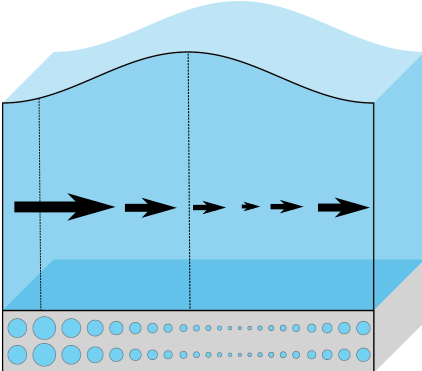
\includegraphics[width=0.5\textwidth]{pictures/schematic_mechanism_unstable.png}
\caption[Schematic showing the phase shift between variables that forces a positive feedback.]{Schematic showing the phase shift between variables that forces a positive feedback. A low in effective pressure (shown by larger pores) and high in ice velocity (at the left hand dotted line) lie upstream from a hump in the ice thickness (right hand dotted line). A decrease in velocity as ice flows through the ice hump will cause the hump to grow. The larger hump routes more water towards a low in effective pressure.}
\label{fig:schematic_unstable}
\end{figure}

%\subsection{Parameter inputs} 

The physical laws and parameters used in this paper are representative of the Antarctic ice sheet. 
The permeability law used falls within bounds of empirical studies which find relationships close to  
$\kappa(N) = \kappa_0 e^ {-m N}, \quad  \kappa_0 = 2.9 \times 10^{-13} \mathrm{   m}^2$ and $m = 5.6 \times 10^{-6} \mathrm{  Pa}^{-1}$ for permeability on a soft bed \citep{boulton1974nature, mckinlay1975representative}. When scaled for the typically low values of effective pressure found in Antarctic ice sheets, $N<100 \mathrm{ kPa}$ \citep{engelhardt1997basal, alley2001west}, permeability is weakly dependent on effective pressure, similar to the relationship above. 
The power sliding law $ \tau_b = u^a N^b $ with $a=b=1/2$ falls within commonly predicted values of $0< a,b <1$ 
\citep{lliboutry1968general, budd1979empirical, bindschadler1983importance, fowler1986sliding, fowler1987sliding, boulton1987sediment, kamb1991rheological, iverson1998ring}.
Water storage ($h_w$) has been found to vary between at least $2 \mbox{ mm}$ \citep{engelhardt1997basal} 
and $2\mbox{ m}$ \citep{tulaczyk2000basal, engelhardt1990physical, kamb1991rheological}.
Scaled for small $[N]$ and $h_w([N])$, the magnitudes for water storage used our simulation lie within this range. 

%kamb finds void ratio, engelhard finds till depth
% Empirical studies confirm Antarctic scales: we choose regieme.
% $rho = 1000;
% rho_w = 900
% g = 10;
% eta= 10^12
% gamma=1e2
% N=10
% theta=0.0001;

% t_yr = 100 days
% u_m/yr =  40
% x = 1000
% k_max= 0.3227
% wavelength max = 19.5$
% corresponds to 20 km.

With a selected set of dimensionless parameters, Equations \eqref{edg} must be satisfied with realistic scales. With five scales and a large realistic range for a number of these, the numerical simulation presented could depict a wide range of regimes. Below is justification for a single regime, selected specifically to represent realistic values. This regime should be taken as an example of conditions that foster an instability, but not as a prediction of how we expect the instability to manifest in reality.

We set constants ice density $\rho$, water density $\rho_w$, and gravity as $1000 \mbox{kgm}^3$, $900\mbox{kgm}^3$ and $g=10 \mbox{ms}^{-2}$ respectively. With an effective pressure scale $ [N]=10 \mbox{ kPa}$ that corresponds to low values typical of areas of fast sliding  \citep{engelhardt1997basal, alley2001west} and, the size of $\gamma=100$  realistically flat bed slope $\theta = 10^{-4}$  \citep{fretwell2013bedmap2} corresponds to a $[x]=1 \mbox{km}$.
This implies the instability has a dominant wavelength of $20 \mbox{km}$, and Figure \ref{fig:instability_float_1} has a domain $200 \mbox{km}$ long.

With a viscosity $\eta= 10^{12} \mathbin{\mathrm{Pa}} \mathbin{\mathrm{s}}$, an $\epsilon = 1$ corresponds to a reasonably fast velocity scale $[u]=40 \mbox{m}/\mbox{yr}$. This implies that in our simulation velocities vary from $30-80\mbox{ma}^{-1}$ This is realistic in Antarctica \citep{rignot2011ice}. Lastly, with $\delta = 1000$, our time scale is $[t]=10.4$ days. This relates to our simulation growing in amplitude to $N=0$ in $5 1/2$ years.  
Lastly a realistic $[h]$ of $2000 \mbox{ m}$ \citep{fretwell2013bedmap2} relates to a 2000m thick ice sheet which shows surface perturbations of around 2m.

\section{Discussion} \label{sec:Discussion}

%\subsection{Summary}

% We have looked at a coupled ice flow--melt drainage model in one horizontal dimension, with the aim of identifying whether any pattern--forming instabilities can appear, and what those 
% instabilities might lead to. We identified one such instability that leads to the formation of patterned `sticky spot'--lake pairs, and described the mechanisms that force the instability: A patch of high water pressure, or low 
% effective pressure, at the bed can lead to faster ice flow that causes
% ice to pile up downstream of the patch, leading to a reduction in 
% hydraulic gradient and hence a reduction in water flux that, in turn, 
% causes water to accumulate where effective pressure is already low. This feedback is related to the relationship between subglacial lakes and ice surface expression described in \cite{sergienko2011sticky}, where an induced slippery spot causes a pile up of ice, and downstream pooling of water. The structure predicted by \citet{sergienko2011sticky} is similar to that simulated in our nonlinear model.

We have confirmed the existence of an instability with a
systematically reduced model (Section \ref{sec: lin_stab_ana}). The instability manifests when bed conditions support a permeability that is only weakly dependent on effective pressure.
%\subsection{DETAIL/BALANCES}
Additionally, the model bed gradient was very small, and
changes in ice thickness were assumed to be very small compared to steady state ice thickness. 
%\subsection{BIFURCATION}
%\subsection{Discussion of results} 

The results of the nonlinear simulation present a number of features of interest.
Firstly, for specific parameter regimes the nonlinear solution is unstable, and grows in amplitude until it reaches zero effective pressure at some point in space. This describes the ice sheet being at the point of flotation: the weight of the ice is supported by the drainage system pressure, not by the bed. At this point the bed and ice sheet could begin to separate to form a deepening subglacial lake. In previous work modelling basal pattern formation by \citet{hindmarsh1998ice} and \citet{fowler2000instability} flotation also occurs, though is formed by feedbacks in sediment transport, not through coupling with the ice sheet.

Secondly, while initial conditions have a large effect on the amplitude of the solution described, the feedback produces a consistent spatial structure:  regions of the nonlinear solution where $N$ becomes small and goes to zero 
are localised, and are separated by larger regions in which $N$ 
has become elevated relative to the effective pressure in the spatially 
uniform steady state. The effect of the instability is that water is taken from larger areas and concentrated in smaller pockets. 
In the nonlinear solution at the point in time where the model ends, illustrated by Figure \ref{fig:solnbreakdown}, mean effective pressure across the domain is $1.0837$, above the steady state average. This does not, however, lead to a net slow--down in ice.  The large--scale effect of the instability is a net speed--up of ice, with an average velocity  of $ u = 1.0296$ when the model reaches flotation.  These values are calculated from a distribution of solutions simulated from random initial conditions (appendix \ref{sec:appen distribution}). With the scale choices discussed above ($[u]=40 \mbox{m}/\mbox{yr}$, $[h] = 2000 \mbox{ m}$), this corresponds to a net increase in the ice flux of $2 370\mbox{m}^2/\mbox{yr}$ over the domain.
Note that we are describing a transitional solution, we cannot describe the long term trend of the distribution of water or velocity without allowing for the continuation of the model in time. This would require a model that allows the formation of deepening lakes under floating ice.  

Thirdly, in accordance with the linearised theory, the pattern continues to move 
upstream as these nonlinear effects manifest themselves.
The wavespeed of the linearised pattern is $ -\Im (\sigma / k )$, only accurate while the pattern is small. In the linear stability analysis (Section \ref{sec: lin_stab_ana} we found the fastest growing Fourier mode to have pattern velocity of $-\Im(\sigma/k) -0.4185$ and growth rate of $\Re ( \sigma )=0.0541 $. The instability will grow to an appreciable size before it moves a long distance relative to a reasonable domain. This is confirmed by the numerical solution.

% \subsection{Limitations and research outlook}

% The model used in this thesis contains some poorly constrained assumptions, primarily regarding water flow at the bed. While we have assumed that relationships governing water storage and permeability are dependent entirely on effective pressure, a more representative model drainage system should  allow for the changing the nature of drainage systems from relatively inefficient distributed drainage networks to form efficient drainage channels, such as that proposed by \citet{hewitt2013seasonal}. 
% With this extension to the drainage model we would expect to see an increase in drainage efficiency in regions of high hydraulic potential gradient. This could potentially exacerbate the instability by creating `R--channels' that could slow ice downstream of areas of low effective pressure, or could slow the feedback by smoothing perturbations in effective pressure more efficiently.
% We note that this extended drainage model still has flaws: in particular, the threshold for channelisation is not well resolved, and the model fails to account for sediment erosion which could also lead to channelisation.

%\subsection{Comparison of results with existing evidence}

%\subsubsection{tiger stripes}
The laterally symmetric `tiger stripes' found by \citet{sergienko2013regular} and \citet{sergienko2014similarity} through inverse modelling are similar in structure to the patterns predicted in Section \ref{sec:numerics} when viewed in one dimension. Both describe striping or oscillating areas of high and low basal shear stress in the downstream direction.  We showed that our model can be realistically scaled to have a dominant wavelength of $19.5 \mathrm{km}$, matching the wavelength observed by \citet{sergienko2014similarity}. It is possible that the stripes identified by \citet{sergienko2014similarity} are formed by an instability similar to that described in this paper. Unlike existing observations, our modeled structures are predicted to migrate upstream. It is feasible that this wave velocity is restricted or `pegged' by fixed spatial changes in bed properties such as variable topography, bed properties or geothermal heatflux.  
%Other mechanisms that could further affect the feedback are sediment transport as modeled in \citet{fowler2014instability}, or thermodynamic feedbacks as in \citet{sergienko2011sticky}.

The `sticky spot'--lake pairs found by \citet{fricker2010synthesizing} in a region of Antarctica are similar to the structures described in this paper. The pairs appear to be quasi--periodic, repeating four times with a wavelength also approximately 20km long perpendicular to the flow direction. These features are modelled by
\citet{sergienko2011sticky}, who prescribe a `sticky--spot' and model consequential lake formation due to a similar feedback mechanisim to that described in this paper. This paper may present a mechanism for the initiation and formation of the sticky--spot feedback that \citet{sergienko2011sticky} prescribe. Additionally, \citet{sergienko2011sticky} found that adding thermodynamic processes to their model further enhanced the instability they modelled.

%\subsubsection{Subglacial lakes}
While this paper does not model the growth of a deepening lake, it predicts the inception of a subglacial lake. Our results suggest that feedbacks could spontaneously distribute water into patterned structures, forming of moving regions of low effective pressure or lakes, on a flat bed. This is in contrast to most of the $379$ subglacial lakes identified in Antarctica, which are large permanent features formed by topographical basins \citep{wright2012fourth}.  While our description of lake formation does not account for these typically large, individual lakes that are generally  observed in practice, it does not attempt to. We have deliberately not introduced basal topography but sought out an instability that forms lakes on a flat bed. Additionally, lakes of the kind we propose would not be detected in altimetry observations looking
for drainage events (rapid, localised surface lowering due to emptying 
of a lake \cite[e.g.][]{siegfried2018thirteen}):
the lakes we describe are unlikely to fill and drain through mechanisms described in j{\"o}kulhlaups models \citep[e.g.][]{nye1976water,evatt2006subglacial}, because our drainage model does not permit channelisation.  

Some identified lakes show very little variation in bed topography, suggesting a large permanent topographic basin is not a prerequisite for lake formation.   While there have been no explicit discoveries of lakes formed from feedbacks in the ice sheet or of migrating lakes, numerous ``fuzzy'' or indefinite lakes suspected to be saturated sediments or ``swamps'' have been found \citep{carter2007radar, young2016distribution}. Similarly, \citet{horgan2012subglacial} theorises that Lake Whillans, Antarctica could be formed and maintained by temporary sediment erosion and deposition based on evidence that the lake has disconnected or transient, active and inactive portions. These kinds of indeterminate lakes may be more representative of the flat bedded water accumulation predicted in this paper. Irrespective of how they formed, it is feasible that the instabilities modelled in this paper catalyse or promote the growth of existing features to form flat bedded lakes similar to Lake Whillans or those described in \citet{fricker2007active}. 

%\subsubsection{Patterns in paleo--ice--sheet remains}

The well documented sediment patterns in paleo--ice sheet remains \citep[e.g.][]{kinahan1872general, hattestrand1997ribbed} such as drumlins, bed ribs or mega scale glacial lineations are not explicitly related to the ice sheet--drainage instability modelled in this paper. Nor are the attempts to model the formation of these features \citep[e.g.][]{hindmarsh1998stability,hindmarsh1998ice, fowler2000instability, schoof2007pressure, dunlop2008bed,fowler2014instability}. We have described a mechanism though which patterns can emerge that is not dependent on models for sediment transport.  As a result, our model cannot simulate the formation of bed--forms. However, it is conceivable that the instability we describe leads to the formation of longitudinally patterned features like drumlins or bed ribs by first making a pattern in basal conditions, creating water--filled cavities at the ice--bed interface spontaneously, and subsequently filling them in with sediments to create the bed--forms.
Using existing or future data sets \citep[e.g.][]{mouginot2017comprehensive} it may be possible to corroborate findings of patterns in this paper by conducting Fourier analysis of Antarctic surface velocities, similar to that conducted on basal data by \cite{spagnolo2017periodic}, but with spatial patterning of velocities in the downstream direction.

\conclusions  %% \conclusions[modified heading if necessary]

This research describes instabilities in the coupling of an ice sheet and its subglacial drainage. We have shown that the instability can cause periodic lakes to spontaneously form under an ice sheet, described the spatial structures produced by the instability, given insight into the mechanisms driving the instabilities, and described conditions that foster an instability.
Describing a coupled ice sheet--drainage system with a  1D model, we used linear stability analysis to find scales and parameters for which a constant steady state solution is unstable.
These scales and parameters describe conditions necessary to force the instability: changes in ice thickness are small, permeability is weakly dependent on effective pressure and the bed slope is small.
Under such conditions, perturbations in the model solution grow in amplitude, developing a periodic spatial structure. Localised lakes (low effective pressure) underlie fast flowing ice, and sit immediately downstream of humps in ice thickness formed by a `sticky spot' (high effective pressure). Similar structures have been described previously in both empirical and modelled research \citep{fricker2010synthesizing,sergienko2011sticky}, 
The instability is driven by a feedback between growing ice humps and localised ponding of water. As the humps grow, water is forced to the upstream side of the hump, reducing basal friction, which in turn increases ice flux into the humps. 
Drawing detailed predictions from the model is not useful due to the broad scale of solutions and lack of empirical justification for parameter inputs. However, the fundamental mechanisms, forces and structure dominating the identified instability are likely key to our understanding of feedbacks in the coupling between ice sheets and subglacial drainage systems. Such feedbacks could play a key role in forming both `sticky spots' and subglacial lakes both of which are important to understanding the dynamics of ice sheets.


% `Sticky spots'  play an role in modulating ice stream flow \citep{winberry2011dynamics}, while it has been hypothesised that subglacial lakes catalyse ice stream inception \citep{pattyn2003new}. 

%% The following commands are for the statements about the availability of data sets and/or software code corresponding to the manuscript.
%% It is strongly recommended to make use of these sections in case data sets and/or software code have been part of your research the article is based on.

\codeavailability{TEXT} %% use this section when having only software code available


\dataavailability{TEXT} %% use this section when having only data sets available


\codedataavailability{TEXT} %% use this section when having data sets and software code available


\sampleavailability{TEXT} %% use this section when having geoscientific samples available

% COMMENT
% \appendix
% \section{Details of Linear Stability Analysis}

% Here we analyse the 
% stability of the steady state solution $(u,h,N) \equiv 
% (\bar{u},\bar{h},\bar{N}) = (1,1,1)$ of the dimensionless coupled 
% ice--flow--drainage model \eqref{scaled_eq_1}--\eqref{scaled_eq_3}. We perturb the solution by writing
% \begin{align}
%   u = \bar{u} + u', \qquad  h = \bar {h} +  h', \qquad N = \bar{N} +  N', 
% \end{align}
% where the primed variables are perturbations, assumed to be small 
% compared with unity. 

% We substitute these into \eqref{eq_1}--\eqref{eq_3}, expanding functions $\tau(u,N)$ and  $\kappa(N) $ as first order Taylor series approximations. Terms of $O(u'^2,h'^2,N'^2)$ or smaller are omitted, resulting in the first order (linear) approximation of our model:
% \begin{align}
%     0 &= 4\epsilon  u'_{xx}- {\tau_b}_u u' - {\tau_b}_N N'+ h' -  \delta h'_x,   \label{Alin_eq_1}\\
%  h'_{t} &= -  u'_{x} - h'_{x}, \label{Alin_eq_2}\\
%  \gamma h_{w N} N'_t &=  - N'_{xx} + r \delta h'_{xx} - \kappa_N N'_x , \label{Alin_eq_3}
%  \end{align}

% where
% $$ \kappa_N = \left.\frac{\partial \kappa}{\partial N}\right|_{N = 
% \bar{N}}, \qquad {\tau_b}_u = \left.\frac{\partial \tau_b}{\partial 
% u}\right|_{u = \bar{u}, N = \bar{N}},  \qquad {\tau_b}_N = 
% \left.\frac{\partial \tau_b}{\partial N}\right|_{u = \bar{u}, N = 
% \bar{N}}. $$
% Note that by construction of the model, we assume that $\kappa_N \leq 
% 0$, $\tau_u \geq 0$, and $\tau_N > 0$.
% Equations \eqref{lin_eq_1}--\eqref{lin_eq_3}
% are a set of linear partial differential equations with constant 
% coefficients posed on a periodic domain, and can be solved by means of a Fourier series \citep{fourier1808memoire}.
%  Thus, we represent the solution in the form
% \begin{align}
% u'(x,t) = \sum_k \hat{u}(t) \exp(ikx), \qquad h'(x,t) = \sum_k 
% \hat{h}(t) \exp(ikx), \qquad  N'(x,t) = \sum_k \hat{N}(t) \exp(ikx),
% \end{align} 
% where the sum is over $k = 2 \pi n/ L$ and $n$ is an integer in the range $(- \infty, \infty)$. 

% Substituting for $u'$, $h'$ and $N'$ and subsequently using the 
% orthogonality of distinct Fourier modes, we obtain
% \begin{align}
%   0 &= \left( -4 \epsilon k^2- \tau_u \right)\hat{u} + \left(  1 - i \right) \hat{h}  -\tau_N \hat{N} ,\\ 
%   \frac{d\hat{h}}{dt} &= - i  k \hat{h} -  i  k \hat{u} ,\\
%   \gamma h_{w N} \frac{d \hat{N}}{d t} &=  \left(  k^2 - i  \kappa_N k \right)\hat{N} -  r \delta k^2 \hat{h} .
%  \end{align}
% This reduces the problem to solving a coupled set of linear, ordinary 
% differential equations with constant coefficients, of the form
% $$
% \mathbf{B}\dot{\mathbf{v}} = \mathbf{A}\mathbf{v},
% $$
% where $\mathbf{B}$ and $\mathbf{A}$ are matrices, and $\mathbf{v} = 
% (\hat{u},\hat{h},\hat{N})^\mathrm{T}$ is the solution vector. Except in the case of a 
% degenerate spectrum, we can write the solution in the form
% \begin{align*}
% \mathbf{v} = \sum_i \mathbf{v}_i \exp(\sigma_i t), 
% \end{align*}
% where each $\sigma_i$ solves the generalised eigenvalue problem
% \begin{align}
% \mathrm{det}(\mathbf{A} - \sigma_i \mathbf{B}) = 0, \label{eigs}
% \end{align}
% and $\mathrm{v}_i$ is the corresponding eigenvector, satisfying 
% $(\mathbf{A} - \sigma_i \mathbf{B})\mathbf{v}_i = \mathrm{0}$.

% Because $\mathbf{A}$ is dependent on wave
% number $k$, we can find a relationship between growth rate $\sigma$ and $k$, $\sigma = \sigma(k)$, known as a dispersion relation. If the real part of $\sigma$ is positive, then the corresponding 
% Fourier mode grows unstably, while a negative real part implies that it 
% will shrink to zero over time. 
% The imaginary part of $-\sigma/k$ gives the wave speed of the associated Fourier mode.

% A single unstable mode $k$ (i.e. a single wavenumber $k$ for 
% which it is possible to find a positive growth rate 
% $\mathrm{Re}(\sigma)$ for a given set of model parameters) signals 
% instability, whereas all wavenumbers must correspond to at least 
% non--positive growth rates to assure stability of a steady state solution.
% In practice, the 
% characteristic equation $\det(\sigma \mathbf{B} - \mathbf{A}) = 
% 0$ defines a quadratic in $\sigma$, and is solveable in closed form. We solve explicitly for the dispersion relation and obtain two roots 
% $\sigma_1(k)$ and $\sigma_2(k)$, given by
% \begin{align}
%  \sigma_{1,2}(k) &=\frac{-b \pm \sqrt{b^2-4a c}}{2a}, \label{full_dispersion_1}
%  \end{align}
%  where
%  \begin{align}
% a &= - 4 \epsilon \gamma h_{w_N}   k^2 - \gamma h_{w_N} \tau_u, \\
% b &=k^2   \tau_u - k \kappa_N \tau_u i - \gamma h_{w_N}    k i - \epsilon    k^3 \kappa_N 4 i +
% 4 \epsilon    k^4   - \delta \gamma h_{w_N}   ^2 k^2 - \gamma h_{w_N} k \tau_u     i - \epsilon \gamma h_{w_N}    k^3     4 i,\\
% c &=   k^2 \kappa_N +    k^3   i + k^2 \kappa_N \tau_u     + k^3   \tau_u i-
%     \delta   ^2 k^3 \kappa_N i + \delta   ^2 k^4   + 4 \epsilon    k^4 \kappa_N     + \epsilon    k^5       4 i -
%     \delta    k^3   r \tau_N i.
%     \label{full_dispersion_4}
% \end{align}


% The analytic solution we find is a linear approximation only valid when close to the steady state $(\bar{u},\bar{h},\bar{N})$.  Assuming a spatially periodic domain with period $L$, we have represented the perturbation away from the steady 
% state $(\bar{u},\bar{h},\bar{N})$ as a Fourier series in the spatial 
% variable $x$. We find that each Fourier mode is the superposition of two 
% eigenfunctions of the eigenvalue problem \eqref{lin_eq_1}--\eqref{lin_eq_3}.
% Specifically:
% \begin{align}
%  \left( \begin{array}{ll}
% u(x,t) \\
% h(x,t) \\
% N(x,t) 
% \end{array} \right)
%  =\left( \begin{array}{ll}
% \bar{u} \\
% \bar{h} \\
% \bar{N} 
% \end{array}\right) +  \sum_{n=-\infty}^{\infty}\left( {c_1}_n
% \mathbf{{v_1}_n} 
%  e^{\sigma_1(k_n)t} + {c_2}_n
% \mathbf{{v_2}_n}
%  e^{\sigma_2(k_n)t} \right) e^{i k_n x}, \label{analytic_solution}
% \end{align}
% where $k_n = 2 \pi n/ L$, $\mathbf{v_{1}}$ and $\mathbf{v_{2}}$ are the eigenvectors that solve equation \eqref{eigs}, and 
% $\sigma_1$ and $\sigma_2$ are the corresponding eigenvalues. 


% Given a point in the space of parameters $\left( \epsilon, \gamma, \delta, h_{w_N}  , \kappa_N, \tau_{b_u}, \tau_{b_N}   \right)$ and wave numbers $(k )$  we can easily calculate the growth rates $\sigma_1$ and $\sigma_2$.
% However, the inverse of this problem, finding the subset of parameters and corresponding wavenumbers
% that generate an instability (at least one root with $\mathrm{Re}(\sigma) > 0$) is not 
% straightforward.
% The argument of the square roots in \eqref{full_dispersion_1} 
% are complex, and although a closed form expression for 
% $\mathrm{Re}(\sigma)$ can be derived, this involves the square root of a 
% combination of terms involving up to the fifth power of $k$.

% Consequently, we further simplify the model 
% to focus on a specific balance of terms in 
% the model, or equally, balance of processes, that produces an unstable solution.
% In finding an unstable parameter regime, we can identify conditions suitable for generating an instability, and are able to deduce the physical mechanism 
% driving that instability.
% We will then return to the full 
% dispersion relation \eqref{full_dispersion_1} to test the predictions of the 
% simplified model we are about derive.

% \section{Numerics}    %% Appendix A

% The numerical simulation (Section \ref{sec:numerics}) uses initial conditions that represent random noise. Using the linear model, we compute eigenvectors for modes of a Fourier series, and sum over them after first multiplying each mode by a random amplitude and phase shift. 

% Our numerical scheme uses operator splitting as seen in \cite{macnamara2016operator}. Let $u^i$, $h^i$ and $N^i$ denote the solutions for $u$, $h$ and $N$ at the $i$th time $t_i$.
%  By `splitting' $\mathbf{v}^i$ where $i$ is the time step, we solve for each variable $u^i, h^i, N^i$ separately and sequentially. 
%  Suppose that $u^{i-1}$, $h^{i-1}$ 
% and $N^{i-1}$ are known, given $h^{i-1}$ and $N^{i-1}$, $u^{i-1}$ can be
% computed from the solution of the elliptic problem \eqref{scaled_eq_1}. At the $i$th time 
% step, we first semi-discretise  equation \eqref{scaled_eq_2} using a backward Euler step to 
% update $h$ from $h^{i-1}$ to $h^i$, treating $u = u^{i-1}$ as fixed. 
% Subsequently, we semi--discretise  equation \eqref{scaled_eq_3} using a backward Euler step in $N$, from $N^{i-1}$ to $N^i$, 
% treating $h = h^{i}$ as fixed. Given the updated $h^i$ and $N^i$, $u^i$ can then 
% again be computed by solving the elliptic problem \eqref{scaled_eq_1}.

% We discretise in space using a finite difference scheme, defining a regular grid of points $x_i$ spaced a distance $\Delta x$ apart.
% Subscripts then indicate the value of a variable at the corresponding grid point, so for 
% instance $u^i_j = u(x_j,t_i)$.
% Under the operator splitting scheme described above, equation \eqref{scaled_eq_1} then becomes
% \begin{align} 
% 4 \epsilon \frac{h_{j+1/2}^i (u^i_{j+1} - u^i_j) - 
% h_{j-1/2}^i (u_j^i - u_{j-1}^i)}{\Delta x^2} - \tau_b(u_j^i,N_j^i) + 
% h_j^i \left( 1- \delta \frac{h_{j+1/2}^i - h_{j-1/2}^i}{\Delta x} \right) 
% &= 0,\label{FD_1}
%  \end{align}
% where we have defined $h$ at half grid points by an algebraic average, $$ h_{j+1/2}^i = (h_{j+1}^i - h_j^i)/2. $$
% Our domain is periodic, and if there are $n$ grid points, then values at a point with spatial subscript $j = n+1$ are identified with their values at $j = 1$.
% Equation 
% \eqref{FD_1} is solved for the $u_j^i$ values. Note that 
% \eqref{FD_1} is nonlinear, and we use Newton's method to 
% solve for the $u_j^i$, using the values $u_j^{i-1}$ from the previous time 
% step as initial guesses where available. In practice, we use a power--law 
% friction law of the form $\tau_b(u,N) =C u^a N^b$.
% %Due to the linear averaging used to find $h$ at half grid points, \eqref{FD_1} has an error of $O(\Delta x)$.

% % The three equations \eqref{scaled_eq_1}, \eqref{scaled_eq_2}, \eqref{scaled_eq_3} are discretised using finite difference methods described below.
% % Subscripts $(\cdot)_j$ denote the spatial step while superscripts $(\cdot)^i$ denote the time step. We find half steps  with an average. $(\cdot)_{j+1 / 2} = \left( (\cdot)_{j+1}-(\cdot)_{j} \right) /2$.
% % Our first equation \eqref{eq_1} is a time independent, elliptic equation, the second \eqref{eq_2} is hyperbolic, and the third \eqref{eq_3} has a diffusive part $ {h_w}_t (N) + N_{xx}=0$.

% Equation \eqref{scaled_eq_2} is 
% semi--discretised in space using a centre difference scheme, and with the operator 
% splitting used here, the backward Euler step for $h$ becomes
% \begin{align}
% h_j^{i+1}= h^i_j - \frac{\Delta t}{2 \Delta x} \left( h^{i+1}_{j+1}u^{i+1}_{j+1} - h^{i+1}_{j-1}u^{i+1}_{j-1} \right), \label{FD_2}
% \end{align}
% which is solved for the $h_j^{i+1}$, using the $u_j^i$ computed previously 
% for given $h_j^i$ and $N_j^i$.
% %Due to the centre difference used, \eqref{FD_2} has a second order error of $O(\Delta x^2)$.

% The operator splitting then goes on to solve for effective pressure 
% $N$. Equation \eqref{scaled_eq_3} is discretised in space using a centred scheme, giving
% \begin{align}
%  \gamma\frac{ h_w \left( N^{i+1}_j \right)- h_w \left( N^{i}_j \right)}{\Delta t} + 
%  &\frac{1}{\Delta x} \kappa \left(  N^{i+1}_{j+1 / 2} \right) \left(  1 + \frac{N^{i+1}_{j+1}-N^{i+1}_{j}}{\Delta x}
%  +r \delta \frac{h^{i+1}_{j+1}-h^{i+1}_{j}}{\Delta x}\right) \nonumber \\
%  - &\frac{1}{\Delta x} \kappa \left(  N^{i+1}_{j-1 / 2} \right) 
%  \left(  1 + \frac{N^{i+1}_{j}-N^{i+1}_{j-1}}{\Delta x}
%  - r \delta \frac{h^{i+1}_{j}-h^{i+1}_{j-1}}{\Delta x}\right)=0. \label{FD_3}
% \end{align}
% Here $N_{j+1/2}^{i+1}$ is again given by an algebraic mean as
% $$ N_{j+1/2}^{i+1} = (N_j^{i+1} + N_{j+1}^{i+1})/2.$$
% We treat the $h_j^{i+1}$ as given by the previous step in the operator 
% splitting, and solve for the $N_j^{i+1}$. As with equation \eqref{FD_1}, equation 
% \eqref{FD_2} is nonlinear in the $N_j^{i+1}$, and we use Newton's method to solve 
% it, using the $N_j^i$ as initial guesses. In practice, we use 
% constitutive relations of the form $h_w(N) = {h_w}_0 e^{-dN}$  and $\kappa(N) = \kappa_0 e^{-mN}$.
% %Due to the linear averaging used to find $h$ at half grid points, \eqref{FD_3} has an error of $O(\Delta x)$.LLL

% The reliability of the solver is confirmed in Figure \ref{fig:nonlin_v_lin1}, where the linear solutions is shown to describes the nonlinear system well while perturbations are small compared with the mean.

% \begin{figure}[htb!]
% \centering
% 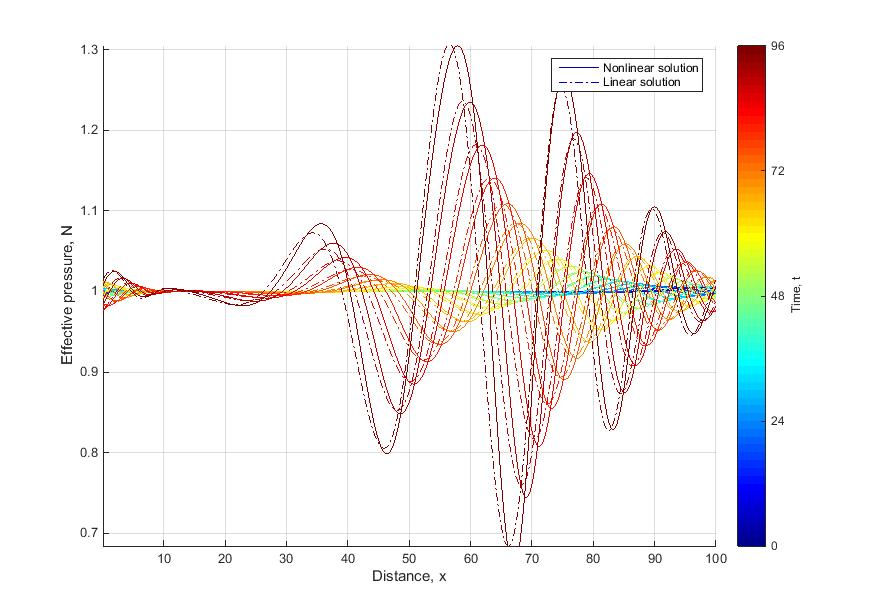
\includegraphics[width=1\textwidth]{pictures/nonlin_v_lin.jpg}
% \caption[Comparison of linear and non linear solutions]{Both linear analytic (Eq. \eqref{analytic_solution}) and nonlinear numeric solutions (Sec. \ref{sec:numerics}) for effective pressure plotted for comparison. Model simulated with $\epsilon= 1, \gamma = 10^{2}, \delta = 10^{3}$ and functions $\tau_b(u,N)= u^{3/4}N^{3/4}, \quad h_w(N)= e^{-N}, \quad \kappa(N)=e^{-0.0001 N}$.  While perturbations from the steady state ($1$) are small, the simulated nonlinear and linear solutions behave the same, confirming the reliability of the nonlinear numerical solver.}
% \label{fig:nonlin_v_lin1}
% \end{figure}

% \subsection{Distribtions} \label{sec:appen distribution}

% In Section \ref{sec:Discussion} we describe average values for evolved variables across the domain. To obtain these, the model was run with random initial conditions. When $N=0$ at a single point, the average value across the domain of each variables was recorded. This was run repeatedly until a smooth distribution of average values was found, plotted below.

% \begin{figure}[htb!]
% \centering
% 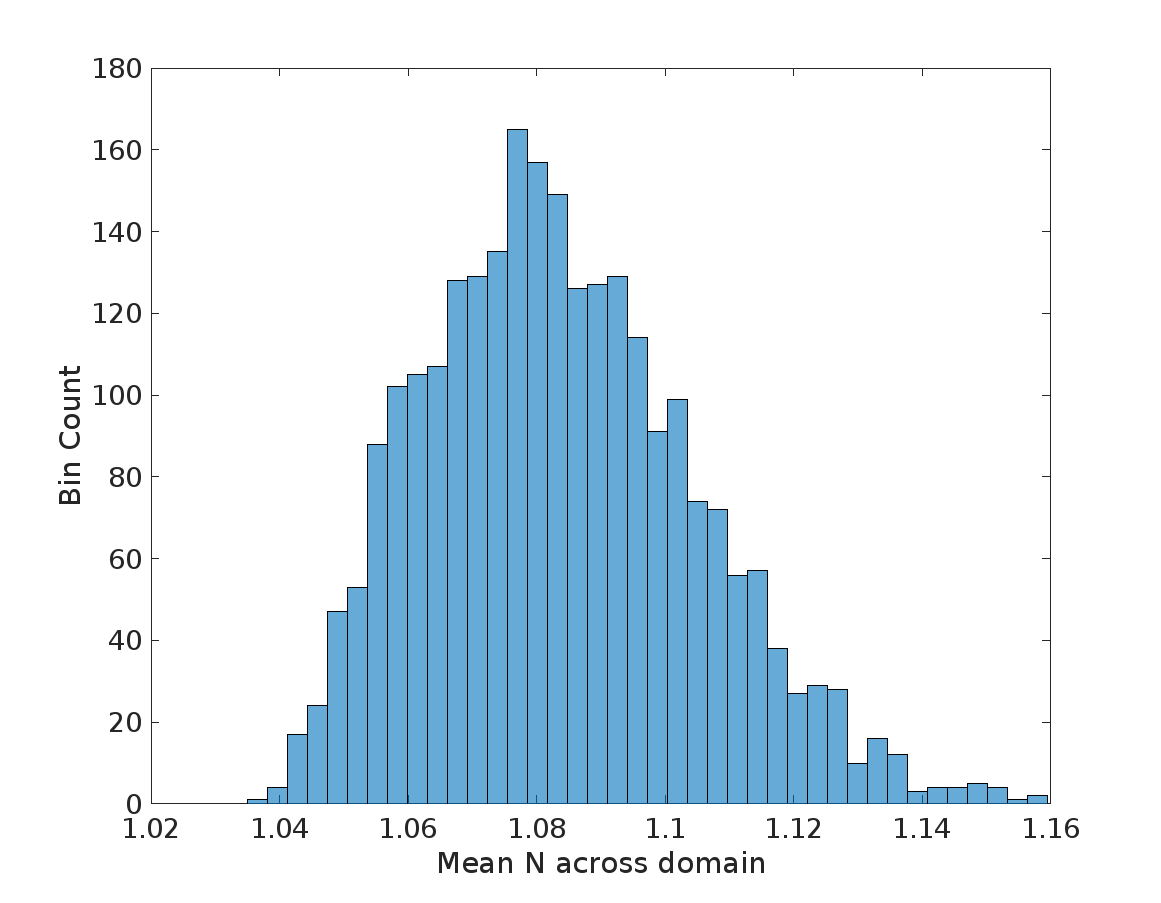
\includegraphics[width=1\textwidth]{pictures/av_distribution_N.png}
% \caption[Distributions of mean effective pressure]{Distribution of mean $N$ across the domain, each simulatation with random initial conditions.}
% \label{distribution}
% \end{figure}

% \noappendix       %% use this to mark the end of the appendix section


%% Regarding figures and tables in appendices, the following two options are possible depending on your general handling of figures and tables in the manuscript environment:

%% Option 1: If you sorted all figures and tables into the sections of the text, please also sort the appendix figures and appendix tables into the respective appendix sections.
%% They will be correctly named automatically.

%% Option 2: If you put all figures after the reference list, please insert appendix tables and figures after the normal tables and figures.
%% To rename them correctly to A1, A2, etc., please add the following commands in front of them:

\appendixfigures  %% needs to be added in front of appendix figures

\appendixtables   %% needs to be added in front of appendix tables

%% Please add \clearpage between each table and/or figure. Further guidelines on figures and tables can be found below.



\authorcontribution{TEXT} %% optional section

\competinginterests{TEXT} %% this section is mandatory even if you declare that no competing interests are present

\disclaimer{TEXT} %% optional section

\begin{acknowledgements}
TEXT
\end{acknowledgements}




%% REFERENCES

%% The reference list is compiled as follows:
\bibliographystyle{copernicus}
\bibliography{patterns_bib.bib}

%% Since the Copernicus LaTeX package includes the BibTeX style file copernicus.bst,
%% authors experienced with BibTeX only have to include the following two lines:
%%
%% \bibliographystyle{copernicus}
%% \bibliography{example.bib}
%%
%% URLs and DOIs can be entered in your BibTeX file as:
%%
%% URL = {http://www.xyz.org/~jones/idx_g.htm}
%% DOI = {10.5194/xyz}


%% LITERATURE CITATIONS
%%
%% command                        & example result
%% \citet{jones90}|               & Jones et al. (1990)
%% \citep{jones90}|               & (Jones et al., 1990)
%% \citep{jones90,jones93}|       & (Jones et al., 1990, 1993)
%% \citep[p.~32]{jones90}|        & (Jones et al., 1990, p.~32)
%% \citep[e.g.,][]{jones90}|      & (e.g., Jones et al., 1990)
%% \citep[e.g.,][p.~32]{jones90}| & (e.g., Jones et al., 1990, p.~32)
%% \citeauthor{jones90}|          & Jones et al.
%% \citeyear{jones90}|            & 1990



%% FIGURES

%% When figures and tables are placed at the end of the MS (article in one-column style), please add \clearpage
%% between bibliography and first table and/or figure as well as between each table and/or figure.


%% ONE-COLUMN FIGURES

%%f
%\begin{figure}[t]
%\includegraphics[width=8.3cm]{FILE NAME}
%\caption{TEXT}
%\end{figure}
%
%%% TWO-COLUMN FIGURES
%
%%f
%\begin{figure*}[t]
%\includegraphics[width=12cm]{FILE NAME}
%\caption{TEXT}
%\end{figure*}
%
%
%%% TABLES
%%%
%%% The different columns must be seperated with a & command and should
%%% end with \\ to identify the column brake.
%
%%% ONE-COLUMN TABLE
%
%%t
%\begin{table}[t]
%\caption{TEXT}
%\begin{tabular}{column = lcr}
%\tophline
%
%\middlehline
%
%\bottomhline
%\end{tabular}
%\belowtable{} % Table Footnotes
%\end{table}
%
%%% TWO-COLUMN TABLE
%
%%t
%\begin{table*}[t]
%\caption{TEXT}
%\begin{tabular}{column = lcr}
%\tophline
%
%\middlehline
%
%\bottomhline
%\end{tabular}
%\belowtable{} % Table Footnotes
%\end{table*}
%
%%% LANDSCAPE TABLE
%
%%t
%\begin{sidewaystable*}[t]
%\caption{TEXT}
%\begin{tabular}{column = lcr}
%\tophline
%
%\middlehline
%
%\bottomhline
%\end{tabular}
%\belowtable{} % Table Footnotes
%\end{sidewaystable*}
%
%
%%% MATHEMATICAL EXPRESSIONS
%
%%% All papers typeset by Copernicus Publications follow the math typesetting regulations
%%% given by the IUPAC Green Book (IUPAC: Quantities, Units and Symbols in Physical Chemistry,
%%% 2nd Edn., Blackwell Science, available at: http://old.iupac.org/publications/books/gbook/green_book_2ed.pdf, 1993).
%%%
%%% Physical quantities/variables are typeset in italic font (t for time, T for Temperature)
%%% Indices which are not defined are typeset in italic font (x, y, z, a, b, c)
%%% Items/objects which are defined are typeset in roman font (Car A, Car B)
%%% Descriptions/specifications which are defined by itself are typeset in roman font (abs, rel, ref, tot, net, ice)
%%% Abbreviations from 2 letters are typeset in roman font (RH, LAI)
%%% Vectors are identified in bold italic font using \vec{x}
%%% Matrices are identified in bold roman font
%%% Multiplication signs are typeset using the LaTeX commands \times (for vector products, grids, and exponential notations) or \cdot
%%% The character * should not be applied as mutliplication sign
%
%
%%% EQUATIONS
%
%%% Single-row equation
%
%\begin{equation}
%
%\end{equation}
%
%%% Multiline equation
%
%\begin{align}
%& 3 + 5 = 8\\
%& 3 + 5 = 8\\
%& 3 + 5 = 8
%\end{align}
%
%
%%% MATRICES
%
%\begin{matrix}
%x & y & z\\
%x & y & z\\
%x & y & z\\
%\end{matrix}
%
%
%%% ALGORITHM
%
%\begin{algorithm}
%\caption{...}
%\label{a1}
%\begin{algorithmic}
%...
%\end{algorithmic}
%\end{algorithm}
%
%
%%% CHEMICAL FORMULAS AND REACTIONS
%
%%% For formulas embedded in the text, please use \chem{}
%
%%% The reaction environment creates labels including the letter R, i.e. (R1), (R2), etc.
%
%\begin{reaction}
%%% \rightarrow should be used for normal (one-way) chemical reactions
%%% \rightleftharpoons should be used for equilibria
%%% \leftrightarrow should be used for resonance structures
%\end{reaction}
%
%
%%% PHYSICAL UNITS
%%%
%%% Please use \unit{} and apply the exponential notation


\end{document}
